\graphicspath{
  {./images/bmps/}{./images/vects/}{./images/}
  {./images/presentation/bmps/}{./images/presentation/vects/}{./images/presentation/}
  {./images/chapter00/bmps/}{./images/chapter00/vects/}{./images/chapter00/}
  {./images/chapter04/bmps/}{./images/chapter04/vects/}{./images/chapter04/}
}

\subsection{Stixel World}

\begin{frame}{Stixel World}
 \begin{itemize}
  \item<1-> Proposed by \cite{badino2009stixel}.
  \item<1-> Representation of the world based on a set of rectangular sticks named \emph{stixels}, defined by:
  \begin{itemize}
   \item<1-> Position relative to the camera
   \item<1-> Height
  \end{itemize}
  
  \item<2->Advantages:
  \begin{enumerate}
   \item<3-> Compact
   \item<4-> Complete
   \item<5-> Stable
   \item<6-> Robust   
  \end{enumerate}
 \end{itemize}

 \note {
 \begin{itemize}
  \item Stixel: from stick and pixel
  \item Stixels stand vertically on the ground
  \item Advantages:
  \begin{itemize}
    \item \emph{Compact}. Significant reduction of the data volume.
    \item \emph{Complete}. Information of interest is preserved.
    \item \emph{Stable}. Small changes of the underlying data must not cause rapid changes within the representation.
    \item \emph{Robust}. Outliers must have minimal or no impact on the resulting representation.
  \end{itemize}
 \end{itemize}
 }
\end{frame}

\begin{frame}{Stixel Tracking}
 \begin{itemize}
  \item Our work is based on \cite{benenson2012fast, gunyel2012stixels}
  \item Contribution:
  \begin{itemize}
    \item<2-> Improvement of the reconstruction quality.
    \item<3-> Improvement of detection results. 
    \item<4-> Different cost metrics tested. 
    \item<5-> Faster tracking.
    \item<6-> Robust after changes between images.
 \end{itemize}
 \end{itemize}

  \note {
  \begin{itemize}
    \item Benenson: 
    \begin{itemize}
      \item No need of a depth map
    \end{itemize}
    \item Improvement of the reconstruction quality obtained by the stixels, specially in terms of the computed depth. Free space computation without the use of a disparity map have some drawbacks. Some of them are related to the fact that precision in the reconstruction of the obstacles is not good enough. Object reconstruction detection scheme proposed in this chapter allows the correction of stixel depths and the removal of some fake obstacles.
    \item Improvement of results obtained by the method described in \cite{gunyel2012stixels}, in both object and two-level tracking approaches. We modified the method by using a graph-based approach instead of a \ac{DP} based method, as they did. 
    \item Different cost metrics for the tracking have been tested, with promising results. 
    \item Faster tracking. Speed achieved with our implementation is higher, specially in the object based tracking. The two-level tracking is also a little bit faster, thanks to the usage of a bipartite graph based method for the matching of the stixels between frames.
    \item Our method is slightly more robust after changes between images (for example, in presence of a low framerate), specially in the case of the approach in which just the object level is used.
  \end{itemize}
  }
\end{frame}

\begin{frame}{Pipeline}
  \begin{center}
    \includegraphics{pipeline_cp04}
  \end{center}
  
  \note {

  }
\end{frame}

\begin{frame}{Tracking}
  We take some assumptions:
  \begin{itemize}
    \item All stixels have been properly estimated.
    \item Maximal speed of the objects is limited.
    \item Small temporal difference between consecutive frames.
  \end{itemize}
  
  \begin{center}
   \includegraphics[width=0.5\textwidth]{stixels_over_original}
  \end{center}

  \note {
  \begin{itemize}
    \item First, we assume that all stixels have been properly estimated.
    \item The maximal speed of the objects is limited, so we limit the search range between stixels to a certain threshold. This range depends on the distance of the stixel at the current frame and the frame rate. As there is just one stixel per column, we can limit also the matching process to a search into the $u$ direction.
    \item There is not a big temporal difference between two consecutive frames. That means that the same stixel at time $t$ and $t - 1$ should look quite similar. Also their height in meters should not change. Txhis temporary consistency is more or less restrictive depending on the approach finally used for the tracking process.
  \end{itemize}
  }
\end{frame}

\begin{frame}{Stixels-level tracking}
  \begin{itemize}
    \item Tracking is performed at stixel level.
    \item Pair matching problem.
    \item Bipartite graph:
    \begin{itemize}
      \item Nodes are the stixels at frames $t$ and $t-1$.
      \item Edges are associated to a motion cost $c_m$.
  \end{itemize}
%   \begin{center}
  \vskip 0.2cm
  \begin{equation}
  \nonumber
    c_m(u_i\{t\}, u_j\{t - 1\}) = 
    \begin{align*}
      \begin{cases}
      f_{cost}(u_i\{t\}, u_j\{t - 1\}) & \textbf{if} \text{ applicable} \\
      \infty & \textbf{otherwise}
      \end{cases}
    \end{align*}
  \end{equation}
%   \end{center}
  \item Matching applicable if:
  \begin{itemize}
    \item $|X(u_i\{t\}) - X(u_j\{t - 1\})| < \tau_{max\_disp}$.
    \item $u_i\{t\}$ is not a new stixel.
    \item $u_i\{t\}$ and $u_j\{t - 1\}$ not occluded.
    \item $f_{cost}(u_i\{t\}, u_j\{t - 1\}) < \tau_{max\_cost}$.
  \end{itemize}
    
  \end{itemize}
  
  \note {
  \begin{itemize}
    \item Pair matching problem $\rightarrow$ Since we want to match each stixel column with a column from the prev. frame.
  \end{itemize}
  \begin{itemize}
    \item $|X(u_i\{t\}) - X(u_j\{t - 1\})| < \tau_{max\_disp}$, where the free parameter $\tau_{max\_disp}$ indicates the maximal displacement of a certain stixel between frames; and $X(u)$ refers to its $X$ position in 3d coordinates.
    \item $u_i\{t\}$ is not a new stixel. That is, this is not the very first frame in which the stixel appears.
    \item Stixels $u_i\{t\}$ and $u_j\{t - 1\}$ are not occluded.
    \item $f_{cost}(u_i\{t\}, u_j\{t - 1\}) < \tau_{max\_cost}$.
  \end{itemize}
  }
\end{frame}

\begin{frame}{Cost function}
  \begin{overlayarea}{\textwidth}{0.5\textheight}
  \only<1> {
  \begin{equation}
    \nonumber \small
    \begin{align*}
    f_{cost}(u_i\{t\}, u_j\{t - 1\}) =~  & & \alpha_{SAD} & ~\cdot~ & f_{SAD}(u_i\{t\}, u_j\{t - 1\}) \\
	& + & \alpha_{hist} & ~\cdot~ & f_{hist}(u_i\{t\}, u_j\{t - 1\}) \\
	& + & \alpha_{height} & ~\cdot~ & f_{height}(u_i\{t\}, u_j\{t - 1\})
    \end{align*}
  \end{equation}
  
  \begin{itemize}
   \item Cost functions:
    \begin{itemize}
      \item Sum of Absolute Differences (SAD) $\rightarrow f_{SAD}(u_i\{t\}, u_j\{t - 1\})$
      \item Histograms matching $\rightarrow f_{hist}(u_i\{t\}, u_j\{t - 1\})$
      \item Height difference $\rightarrow f_{height}(u_i\{t\}, u_j\{t - 1\})$
    \end{itemize}
  \end{itemize}
  }
  \only<2>{
  \vskip 1cm
  \begin{block}{Solve}
      \begin{center}
	\resizebox{.6\hsize}{!}{$\mathcal{\hat{M}}=\underset{\mathcal{M}}{\arg\min} \underset{(i, j) \in \mathcal{M}}{\sum} \omega_{i,j}, ~~~~\exists! (i, \cdot) \wedge \exists! (\cdot, j)$}
      \end{center}
    \end{block}
  }
  \end{overlayarea}
  
  \begin{center}
    \includegraphics[width=0.75\textwidth]{bipartite_graph}
  \end{center}
  
  \note {
    Here, $\alpha_{SAD} + \alpha_{hist} + \alpha_{height} = 1$.
    \begin{itemize}
      \item Sum of Absolute Differences (SAD):
      \begin{itemize}
       \item Pixel-wise \acl{SAD} over the RGB color scheme between $u_i\{t\}$ and $u_j\{t - 1\}$
       \item As it is very unlikely for a candidate pair of stixels to have the exact same height, they are resized to a dimension of $30\,px$.
       \item This metric was originally used in \cite{gunyel2012stixels} for the computation of the movement of the stixels.
      \end{itemize}
      \item Histograms matching (Hellinger distance):
      \begin{itemize}
       \item The size of a certain stixel changes slightly between frames (the position of the object partially represented by the stixel changes its depth in the scene, or noise in the height detection of the stixel)
       \item In order to normalize this, we compute the histogram of each of the stixels being compared. 
       \item The cost is computed as the Hellinger distance between both histograms
      \end{itemize}
      \item Height difference:
      \begin{itemize}
       \item This metric is used to complement the other two metrics (by its own is not enough to do a matching), but it is good enough to help in the decision, in case of very similar scores in two or more possible matches.
       \item 
      \end{itemize}
      \item In our tests, we have tried different values for $\alpha_{SAD}$, $\alpha_{hist}$ and $\alpha_{height}$, obtaining the results shown, both in terms of performance and time. 
      \item The value obtained using the function $f_{cost}$ is used to weight the links between the nodes of a bipartite graph.  \item In the top row, we can see the nodes (stixels) at current time, while in the lower row, previous stixels are shown. \item Costs of the match are associated to the edges, depicted in the image with the notation $\omega_{i,j}$.
      \item Over this graph, we solve the minimization problem
      \item This problem is solved using a $O(n \cdot m \cdot log(n))$ implementation of the Edmond's maximum weighted matching algorithm
      \item Advantages: ensures that a stixel is matched with \emph{just one} stixel in the other frame; Faster.
    \end{itemize}
  }
\end{frame}


\begin{frame}{Obstacle-level tracking}
  \begin{enumerate}
    \item Object detection.
    \begin{itemize}
     \item Clustering.
     \item Aggregation.
     \item Filtering.
    \end{itemize}

    \item Object tracking.
  \end{enumerate}
  
  \note {
  \begin{itemize}
    \item In this stage, we perform the tracking at obstacle level. 
    \item In the case of two-level tracking, we have a set of matchings, which relates each stixel at column $u_i$ in the frame $t$ with the stixel at column $u_j$ in the frame $t - 1$. 
    \item In the other approach, we do not really need to have these matches for this stage, as the tracking is done directly at this level. 
  \end{itemize}
  }
\end{frame}

\begin{frame}{Obstacle-level tracking}
  \framesubtitle{Object detection}
  \begin{itemize}
    \item<1-> Clustering.
    \item<2-> Aggregation.
    \item<3-> Filtering.
  \end{itemize}
  \begin{overlayarea}{\textwidth}{\textheight}
    \only<3>{    
    \vskip-0.75cm
    \begin{algorithm}[H]
      \begin{algorithmic}[1]
      \footnotesize
      \Function{Clustering}{$\mathcal{Q}\{t\}$}
	\State {$\mathcal{O} \gets \emptyset$}
	\State {$o \gets \emptyset$}
	\For {\textbf{each} stixel $q_i \in \mathcal{Q}$, from left to right}
	  \If {$|depth(q_i) - depth(q_{i-1})| > \tau_{depth\_dist}$}
	    \If {$|depth(q_i) - depth(q_{i-1})| > \tau_{depth\_dist}$}
	      \State {$width(o) > \tau_{min\_width}$}
	    \EndIf
	    \State {$o \gets \emptyset$}
	  \EndIf
	  \State {$o \gets o \cup q_i$}
	\EndFor
      \EndFunction
      \end{algorithmic}
      \end{algorithm}
    }
    \only<4>{
    \begin{figure}
      \includegraphics[width=0.5\textwidth]{obstaclesBeforeAggregation}
    \end{figure}
    }
    \only<5>{
    \vskip-0.75cm
    \begin{algorithm}[H]
      \begin{algorithmic}[1]
	\footnotesize
	\Function{Aggregation}{$\mathcal{O}$}
	\State {$\mathcal{O'} \gets \emptyset$}
	\State {$o' \gets \emptyset$}
	\For {\textbf{each} object $o_i \in \mathcal{O}$, from left to right}
	  \If {$|X(o_i) - X(o_{i-1})| > \tau_{lateral\_aggregation\_dist}$ \textbf{or}\\ \indent\indent\indent
	      $|Z(o_i) - Z(o_{i-1})| > \tau_{depth\_dist}$ \indent\indent~}

	    \State {$\mathcal{O} \gets \mathcal{O} \cup o'$}
	    \State {$o' \gets \emptyset$}
	  \EndIf
	  \State {$o' \gets o' \cup o$}
	\EndFor
      \EndFunction
      \end{algorithmic}
      \end{algorithm}
    }
    \only<6>{
    \begin{figure}
      \includegraphics[width=0.5\textwidth]{obstaclesAggregated}
    \end{figure}
    }
  \end{overlayarea}
  
  \note {
  \begin{itemize}
   \item Clustering
   \begin{itemize}
    \item At the end of the process, we will have got the set of obstacles $o_i \in \mathcal{O}$. 
    \item Each obstacle has several parameters associated. 
    \item One of them is the depth, which is computed as the minimal depth from all the clustered stixels.
   \end{itemize}
   \item Aggregation
  \begin{itemize}
    \item In certain cases, due to a bad detection, some stixels are wrongly located at a depth different from their real position.
    \item Final depth of the obstacle is computed as the minimal depth of the original obstacles.
   \end{itemize}

  \end{itemize}

  
  }
\end{frame}

\begin{frame}{Obstacle-level tracking}
  \framesubtitle{Polar rectification}
  \begin{itemize}
    \item<1-> Correspondences between epipolar lines $\rightarrow$ Matrix $H$.
    \item<2-> Common region between images.
    \item<3-> Rectification.
  \end{itemize}
  \begin{overlayarea}{\textwidth}{\textheight}
    \only<1>{
    \begin{figure}
      \includegraphics[height=0.6\textheight]{fundamentalMatrixComputation}
    \end{figure}
    }
    \only<2>{
    \begin{figure}
      \includegraphics[width=\textwidth]{polar_common_region}
    \end{figure}
    }
    \only<3>{
    \begin{figure}
      \centering
      \begin{tabular}{ cc }
	\includegraphics[height=0.6\textheight]{polarRectification}\label{fig:cp04_polarRectification} &
	\includegraphics[height=0.6\textheight]{polarDiff}\label{fig:cp04_polarDiff}
      \end{tabular}
    \end{figure}
    }
    \end{overlayarea}
  \note {
  
  }
\end{frame}

\begin{frame}{Obstacle-level tracking}
  \framesubtitle{Polar rectification}
  \begin{itemize}
    \item<1-> Correspondences between epipolar lines $\rightarrow$ Matrix $H$.
    \item<2-> Common region between images.
    \item<3-> Rectification.
  \end{itemize}
  \begin{overlayarea}{\textwidth}{\textheight}
    \only<1>{
    \begin{figure}
      \includegraphics[height=0.6\textheight]{fundamentalMatrixComputation}
    \end{figure}
    }
    \only<2>{
    \begin{figure}
      \includegraphics[width=\textwidth]{polar_common_region}
    \end{figure}
    }
    \only<3>{
    \begin{figure}
      \centering
      \begin{tabular}{ cc }
	\includegraphics[height=0.6\textheight]{polarRectification}\label{fig:cp04_polarRectification} &
	\includegraphics[height=0.6\textheight]{polarDiff}\label{fig:cp04_polarDiff}
      \end{tabular}
    \end{figure}
    }
    \end{overlayarea}
  \note {
  
  }
\end{frame}

\begin{frame}{Obstacle-level tracking}
  \framesubtitle{Obstacle filtering}

  \begin{figure}
    \begin{minipage}{\textwidth}
      \centering
      \includegraphics[width=0.5\textwidth]{thresholdedPolar}
      \end{minipage}\hfill~
    \begin{minipage}{\textwidth}
      \centering
      \begin{tabular}{ |c|c|c|c|c|c|c|c|c|c|c|}
	\hline
	\includegraphics[width=0.075\textwidth, height=0.075\textwidth]{obstacleFilter/roi0} &
	\includegraphics[width=0.075\textwidth, height=0.075\textwidth]{obstacleFilter/roi1} &
	\includegraphics[width=0.075\textwidth, height=0.075\textwidth]{obstacleFilter/roi2} &
	\includegraphics[width=0.075\textwidth, height=0.075\textwidth]{obstacleFilter/roi3} &
	\includegraphics[width=0.075\textwidth, height=0.075\textwidth]{obstacleFilter/roi4} & 
	\includegraphics[width=0.075\textwidth, height=0.075\textwidth]{obstacleFilter/roi5} &
	\includegraphics[width=0.075\textwidth, height=0.075\textwidth]{obstacleFilter/roi6} &
	\includegraphics[width=0.075\textwidth, height=0.075\textwidth]{obstacleFilter/roi7} &
	\includegraphics[width=0.075\textwidth, height=0.075\textwidth]{obstacleFilter/roi8} &
	\includegraphics[width=0.075\textwidth, height=0.075\textwidth]{obstacleFilter/roi9} &
	\includegraphics[width=0.075\textwidth, height=0.075\textwidth]{obstacleFilter/roi10} \\
	\hline
	\setlength{\fboxsep}{1pt}\fcolorbox{green}{green}{\includegraphics[width=0.075\textwidth, height=0.075\textwidth]{obstacleFilter/occ0}} &
	\setlength{\fboxsep}{1pt}\fcolorbox{green}{green}{\includegraphics[width=0.075\textwidth, height=0.075\textwidth]{obstacleFilter/occ1}} &
	\setlength{\fboxsep}{1pt}\fcolorbox{green}{green}{\includegraphics[width=0.075\textwidth, height=0.075\textwidth]{obstacleFilter/occ2}} &
	\setlength{\fboxsep}{1pt}\fcolorbox{red}{red}{\includegraphics[width=0.075\textwidth, height=0.075\textwidth]{obstacleFilter/occ3}} &
	\setlength{\fboxsep}{1pt}\fcolorbox{red}{red}{\includegraphics[width=0.075\textwidth, height=0.075\textwidth]{obstacleFilter/occ4}} & 
	\setlength{\fboxsep}{1pt}\fcolorbox{green}{green}{\includegraphics[width=0.075\textwidth, height=0.075\textwidth]{obstacleFilter/occ5}} &
	\setlength{\fboxsep}{1pt}\fcolorbox{red}{red}{\includegraphics[width=0.075\textwidth, height=0.075\textwidth]{obstacleFilter/occ6}} &
	\setlength{\fboxsep}{1pt}\fcolorbox{green}{green}{\includegraphics[width=0.075\textwidth, height=0.075\textwidth]{obstacleFilter/occ7}} &
	\setlength{\fboxsep}{1pt}\fcolorbox{red}{red}{\includegraphics[width=0.075\textwidth, height=0.075\textwidth]{obstacleFilter/occ8}} &
	\setlength{\fboxsep}{1pt}\fcolorbox{green}{green}{\includegraphics[width=0.075\textwidth, height=0.075\textwidth]{obstacleFilter/occ9}} &
	\setlength{\fboxsep}{1pt}\fcolorbox{red}{red}{\includegraphics[width=0.075\textwidth, height=0.075\textwidth]{obstacleFilter/occ10}} \\
	\hline
      \end{tabular}
    \end{minipage}\hfill
  \end{figure}

  \note {
  \begin{itemize}
   \item Using the aligned images, we get the pixelwise SAD of both images, so we can detect pixels for which there are changes.
   \item Difference image is projected back to the current image coordinates.
   \item Difference is binarized, and noise rejected.
   \item For each \ac{ROI}, we reject the top half of it, so we just look for movement in the area of the obstacle that is touching the ground. There are two reasons for that: 
   \begin{enumerate}
    \item the first one is that obstacles that move over the ground usually present more movement in their lower half (for instance, legs or wheel movements). In the case of static obstacles, the movement due to the camera change is more or less similar in the whole object, so we are not loosing information. 
    \item The second reason is that the stixels reconstruction assumes a planar ground in front of the camera, and that they are lying on it. As there should not be changes due to perspective over this planar ground, it is easier to do a discrimination in those areas.
   \end{enumerate}
   \item Image at frame $t$ is registered with frame $t - k$.
   \item For each ROI, we look for motion in the lower half.
   \item The region is divided in real world coordinate cells.
   \begin{itemize}
     \item If there is a point in a cell, it is marked as occupied.
     \item An obstacle is rejected if $fake(o) = true$
   \end{itemize}
  \end{itemize}

  }
\end{frame}

\begin{frame}{Obstacle-level tracking}
  \framesubtitle{Tracking}
  \begin{enumerate}
   \item<1-> Two-level tracking
   \begin{itemize}
    \item<3-> Tracking problem as a pair matching process
    \item<4-> $C_{|\mathcal{O}\{t\}| \times |\mathcal{O}\{t - 1\}|}$
    \item<5-> Two objects are associated if:
    \begin{itemize}
     \item<5-> There is at least one stixel.
     \item<6-> They are close enough.
    \end{itemize}
   \end{itemize}
   \item<2-> Object tracking
  \end{enumerate}
  \begin{overlayarea}{\textwidth}{\textheight}
  \only<4> {
    \vskip-2.0cm
    \begin{block}{Algorithm}
    \vskip-0.4cm
    \begin{algorithm}[H]
    \begin{algorithmic}[1]
    \footnotesize
    \Function{Tracking}{$\mathcal{O}\{t\}$, $\mathcal{O}\{t - 1\}$}
      \State {$C_{|\mathcal{O}\{t\}| \times |\mathcal{O}\{t - 1\}|} \gets 0$}
      \For {\textbf{each} object $o\{t\} \in \mathcal{O}\{t\}$}
	\For {\textbf{each} stixel $q\{t\} \in o$}
	  \State {Find correspondence $q\{t - 1\}$ for $q\{t\}$}
	  \State {Find the object $o\{t - 1\} \in \mathcal{O}\{t - 1\}$ associated to $q\{t - 1\}$}
	  \If {$o\{t - 1\}$ found \textbf{and} $\|o\{t\} - o\{t - 1\}\| < \tau_{max\_obst\_dist}$}
	    \State {$C(o\{t\}, o\{t - 1\}) \gets C(o\{t\}, o\{t - 1\}) + 1$}
	  \EndIf
	\EndFor
      \EndFor
    \EndFunction
    \end{algorithmic}
    \end{algorithm}
    \end{block}
  }
  \only<7> {
    \vskip-1.0cm
    \begin{block}{Minimization problem - Two-level tracking}
      \begin{center}
	\resizebox{.6\hsize}{!}{$\mathcal{\hat{C}}=\underset{\mathcal{C}}{\arg\max} \underset{(i, j) \in \mathcal{M}}{\sum} C(i,j), ~~~~\exists! (i, \cdot) \wedge \exists! (\cdot, j)$}
      \end{center}
    \end{block}
  }
  \only<8> {
%     \vskip-1.0cm
    \begin{block}{Minimization problem - Object tracking}
      \begin{center}
	\resizebox{.8\hsize}{!}{$C(o\{t\}, o\{t - 1\}) = 1 - \left ( 2 \cdot \sqrt { 1 - \underset{i=1}{\overset{d}{\sum}}\sqrt{H(o\{t\})[i] \cdot H(o\{t - 1\})[i]}} \right )$}
      \end{center}
    \end{block}
  }
  \end{overlayarea}

  \note {

  }
\end{frame}

\begin{frame}{Summary}
 \begin{figure}
  \includemovie[autoplay, repeat, controls]{\textwidth}{0.8\textheight}{/home/nestor/Seafile/Videos/Tesis/cp03/ncc.avi}
 \end{figure}
\end{frame}

\begin{frame}{Obstacle detection and tracking}
  \begin{itemize}
  \item Goals:
    \begin{enumerate}
      \item Good obstacle detection rate. \only<2->{\textcolor{green}{\cmark}}
      \item Obstacle localization. \only<3->{\textcolor{green}{\cmark}}
      \item Real time. \only<4->{\textcolor{green}{\cmark}}
      \item Environment conditions independence. \only<5->{\textcolor{green}{\cmark}}
      \item Tracking capabilities. \only<6->{\textcolor{green}{\cmark}}
      \item Moving cameras. \only<7->{\textcolor{green}{\cmark}}
    \end{enumerate}
  \end{itemize}
\end{frame}